%\chapter{Proof of Concept Design and Implementation}
%\chapter{Pixel-based Synthesis of 360\degree Viewpoints}
%\chapter{Pixel-based Synthesis of 360\degree Viewpoints with 2DoF}
\chapter{Pixel-based Rendering of 360\degree Viewpoints with 2DoF}
\section{Approach}
%\begin{itemize}
%  \item most other approaches rely on either geometry or correspondences
%  \item usually some form of triangulation
%  \item use of sphere for ray tracing, then use texture lookup to find the pixel values
%  \item combination of reprojection ie warping with angle constraint and flow-based blending
%  \item first part relies on radius/scale, but no geometry, second part relies on image correspondences
%  \item ``view-dependent texture maps'' \ar environment map / viewpoint is chosen based on some kind of proximity to the synthesized view
%  \item pixel-based, in that each pixel is calculated separately, there are not image-area based constraints
%\end{itemize}

\subsection{Assumptions}
\begin{itemize}
  \item all images are oriented the same
  \item all images were captured on a plane parallel to the floor
  \item the positions of the captures are known
  \item the scale (radius) of the scene is known
  \item all synthesized viewpoints are located inside the scene boundaries
\end{itemize}

\subsection{Basic 2DoF Synthesis}
With these assumptions and using a basic model geometry with the same scale as the captured scene, it is already possible to synthesize new views of approximate to exact accuracy, depending on the scene. The process for basic 2 degree of freedom synthesis presented is a combination of texture-lookup through raytracing, and mosaicking by using a deviation angle constraint.

\subsubsection{Raytracing-based Texture Remapping}
The first step is to remap the texture (i.e. pixel values) of an existing viewpoint to a new viewpoint according to its position in the scene. Theoretically, any 360\degree viewpoint can be remapped to any other, since each 360\degree image captures each point in the scene. This is only theoretically the case, since resolution and occlusions in the scene will conceal some areas for some viewpoints whereas they are visible for others. However, at this point, this will be ignored and it will be assumed that each viewpoint image contains all the points of the scene albeit at different image coordinates and different sampling rates\footnote{Areas closer to the camera are captured with higher sampling rates than areas farther away.}. 

Furthermore, a 3D geometry is needed for calculating ray-scene intersections. Since the approach in this thesis does not capture or infer any real geometry, a model geometry is used that has approximately the same scale as the scene that was captured. The model geometry used is a sphere, as this is a simple, very general geometry to represent a variety of different scenes. The radius of the sphere is chosen so that the sphere contains all possible points in the scene, for which the scale of the scene needs to be known. Under these assumptions, it is possible to remap the image at one viewpoint to a different position.

% This is visualized in Figure~\ref{fig:reflected_rays} a: Each point P of the scene reflects light rays in all directions. These light rays are captured at different viewpoints and are discretized into pixels in the image taken at that viewpoint. As a result, the pixels representing point P are present in the images captured at each viewpoint. This means that when synthesizing a new viewpoint S, the pixels representing point P can theoretically be retrieved from any of the images at the captured viewpoints (Figure~\ref{fig:reflected_rays} b).

In order to do this, several steps of raytracing are necessary, which are visualized in Figure~\ref{fig:raytracing}. Figure~\ref{fig:raytracing} a shows how a camera at a specific viewpoint captures the light rays reflected from the objects in the scene. The captured pixel values are visualized on a circle around the center of projection of the camera (for simplicity's sake, only one row of pixels is shown). Once the viewoints have been captured (there is only one in this example), a new viewpoint is ready to be synthesized. The model geometry is visualized as a circle in Figure~\ref{fig:raytracing} b, with the new viewpoint to be synthesized represented by a dotted circle around a center of projection. For each pixel of the synthesized image, a ray is projected into the scene (Figure~\ref{fig:raytracing} c) and its intersection with the scene is calculated. Then, the ray from the center of projection of the captured viewpoint to the scene intersection is calculated and the pixel value at that position in world coordinates is retrieved (Figure~\ref{fig:raytracing} e) and copied back to the new viewpoint (Figure~\ref{fig:raytracing} f). This way, the pixel values (i.e. texture) of a captured viewpoint are remapped to the new viewpoint (Figure~\ref{fig:raytracing} g). Figure~\ref{fig:raytracing} compares the remapped values to the actual scene. It is immediately visible that

\begin{figure}
\centering
    \hfill
    \begin{subfigure}[t]{0.3\textwidth}            
            \centering
            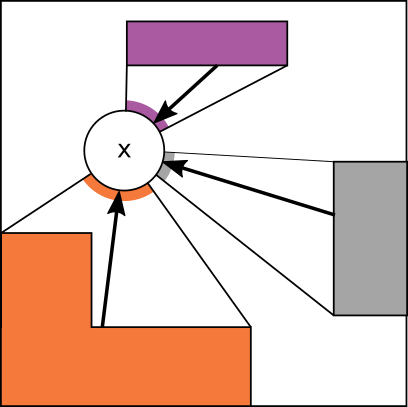
\includegraphics[width=0.9\textwidth]{03/raytracing01.png}
            \caption{The real scene viewed from above: The camera captures light rays reflecting from objects}
    \end{subfigure}%
    \hfill
     %add desired spacing between images, e. g. ~, \quad, \qquad etc.
      %(or a blank line to force the subfigure onto a new line)
    \begin{subfigure}[t]{0.3\textwidth}
            \centering
            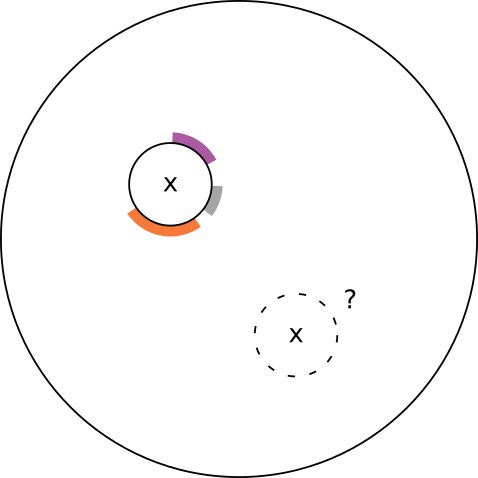
\includegraphics[width=0.9\textwidth]{03/raytracing02.png}
            \caption{A new viewpoint to be synthesized using the model geometry (sphere)}
    \end{subfigure}
    \hfill
    \hfill

    \hfill
    \begin{subfigure}[t]{0.3\textwidth}            
            \centering
            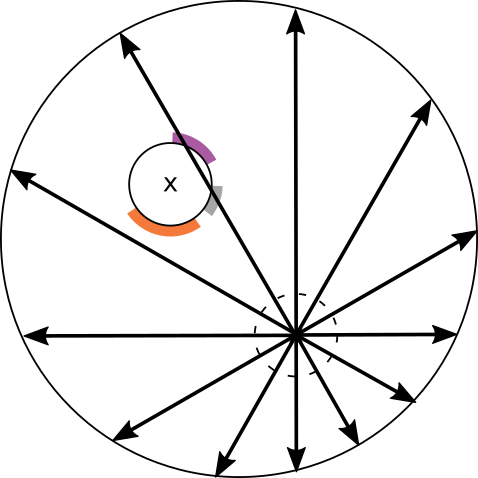
\includegraphics[width=0.9\textwidth]{03/raytracing03.png}
            \caption{A ray for each pixel in the synthesized viewpoint is traced to its intersection with the model}
    \end{subfigure}%
    \hfill
    \begin{subfigure}[t]{0.3\textwidth}
            \centering
            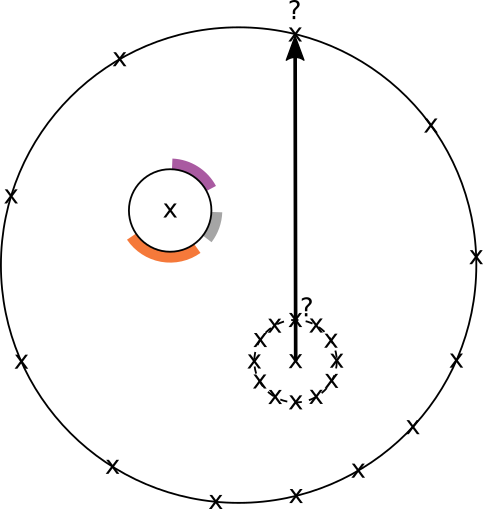
\includegraphics[width=0.9\textwidth]{03/raytracing04.png}
            \caption{For each ray, a texture lookup is performed}
    \end{subfigure}
    \hfill
    \begin{subfigure}[t]{0.3\textwidth}
            \centering
            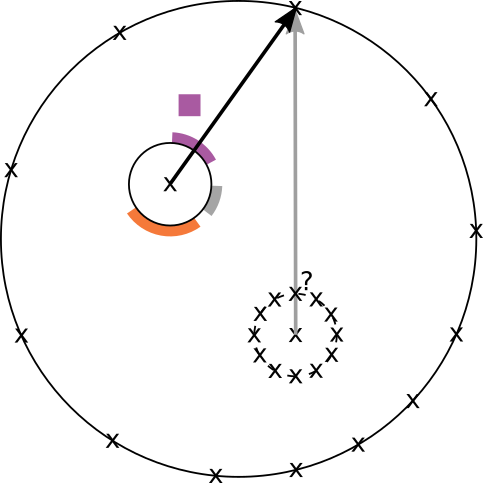
\includegraphics[width=0.9\textwidth]{03/raytracing05.png}
            \caption{From the ray-model intersection, a second ray is traced to the center of projection of the captured viewpoint and the pixel value is looked up}
    \end{subfigure}
    \hfill

    \hfill
    \begin{subfigure}[t]{0.3\textwidth}            
            \centering
            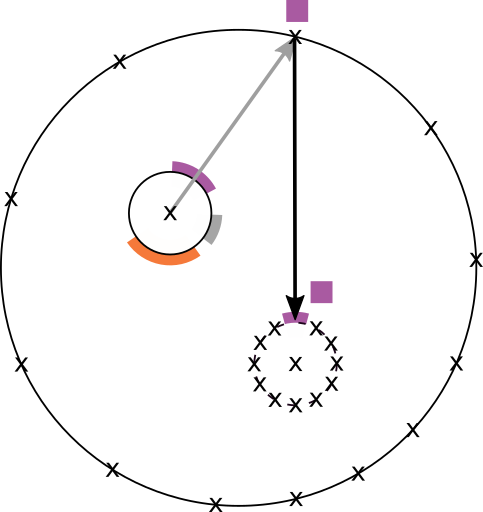
\includegraphics[width=0.9\textwidth]{03/raytracing06.png}
            \caption{The pixel value is copied back to the new viewpoint}
    \end{subfigure}%
    \hfill
    \begin{subfigure}[t]{0.3\textwidth}
            \centering
            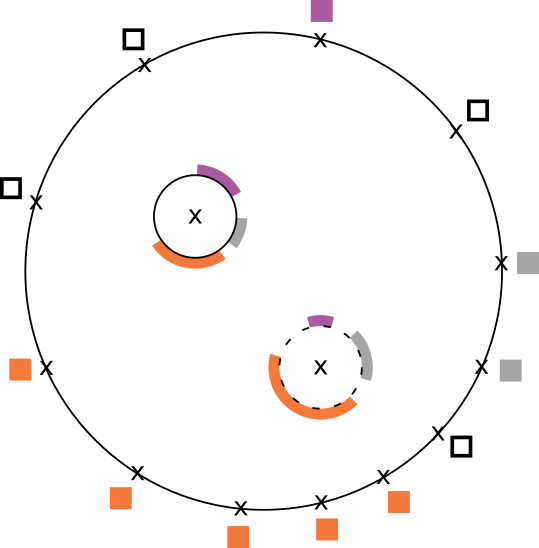
\includegraphics[width=0.9\textwidth]{03/raytracing07.png}
            \caption{This process is repeated for all pixels}
    \end{subfigure}
    \hfill
    \begin{subfigure}[t]{0.3\textwidth}
            \centering
            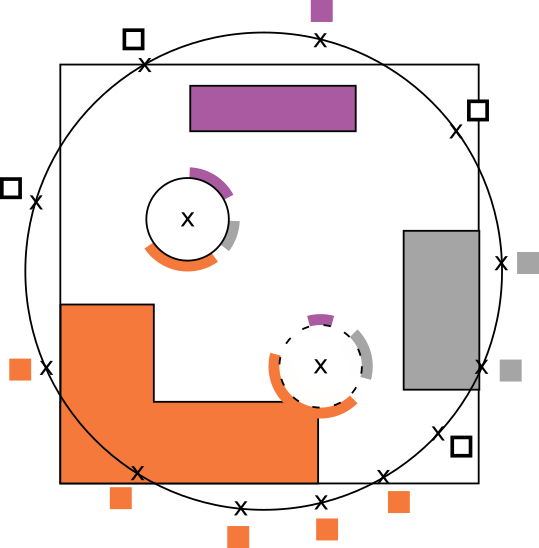
\includegraphics[width=0.9\textwidth]{03/raytracing08.png}
            \caption{The resulting texture mapping from the captured viewpoint to the model geometry in comparison with the original scene}
    \end{subfigure}
    \hfill
    \caption[Process of texture lookup through raytracing]{Process of texture lookup through raytracing}\label{fig:raytracing}
\end{figure}


\paragraph{Ray-sphere intersection}
The vectors representing these rays can be easily derived from the \emph{world coordinates} of the image (see~Section~\ref{fundamentals_360}).

The intersections of these rays with the model geometry can be calculated analytically: The sphere representing the scene can be represented implicitly by Equation~\ref{eq:rsi_spherefull}. The set of points P defined by this equation make up the surface of the sphere (Equation~\ref{eq:rsi_sphereP}). 
The equation describing any point on the ray can be expressed by Equation~\ref{eq:rsi_point}, where $O$ is the origin of the ray, which is the center of projection of the new viewpoint, $t$ is the length of the ray and $D$ is a unit vector describing the direction. 

\begin{align}
  x^2 + y^2 + z^2 - R^2 = 0&\label{eq:rsi_spherefull}\\ 
  P^2 - R^2 = 0&\label{eq:rsi_sphereP}
\end{align} 
\begin{align}
  P = O + tD& \label{eq:rsi_point}
\end{align} 

The point $P$ in Equation~\ref{eq:rsi_sphereP} can be substituted with the equation of the any point on the ray which yields Equation~\ref{eq:rsi_sub}. This equation can be developed into Equation~\ref{eq:rsi_quad}, which is a quadratic function with $a = D^2$, $b = 2OD$, $c = O^2-R^2$ (Equation~\ref{eq:quadf}).

\begin{align}
  |O + tD|^2 - R^2 &= 0  \label{eq:rsi_sub}\\
  D^2 t^2 + 2ODt + O^2 - R^2 &= 0 \label{eq:rsi_quad}
\end{align}

\begin{align}
  a = D^2, b = 2OD, c = O^2-R^2 \\
  f(t) = at^2 + bt + c \label{eq:quadf}\\
  t = \frac{-b \pm \sqrt{b^2 - 4ac}}{2a} \label{eq:solvequadf}
\end{align}

This equation can then be solved for t. Since the radius of the sphere is chosen so that it contains the complete scene and no viewpoints are synthesized outside of the scene, the quadratic function will always have two solutions (i.e. two intersections): one for which the vector length $t$ is negative, and one for which the vector length is positive. The positive value is used to find the intersection in question.


%\begin{figure}[]
%\centering
%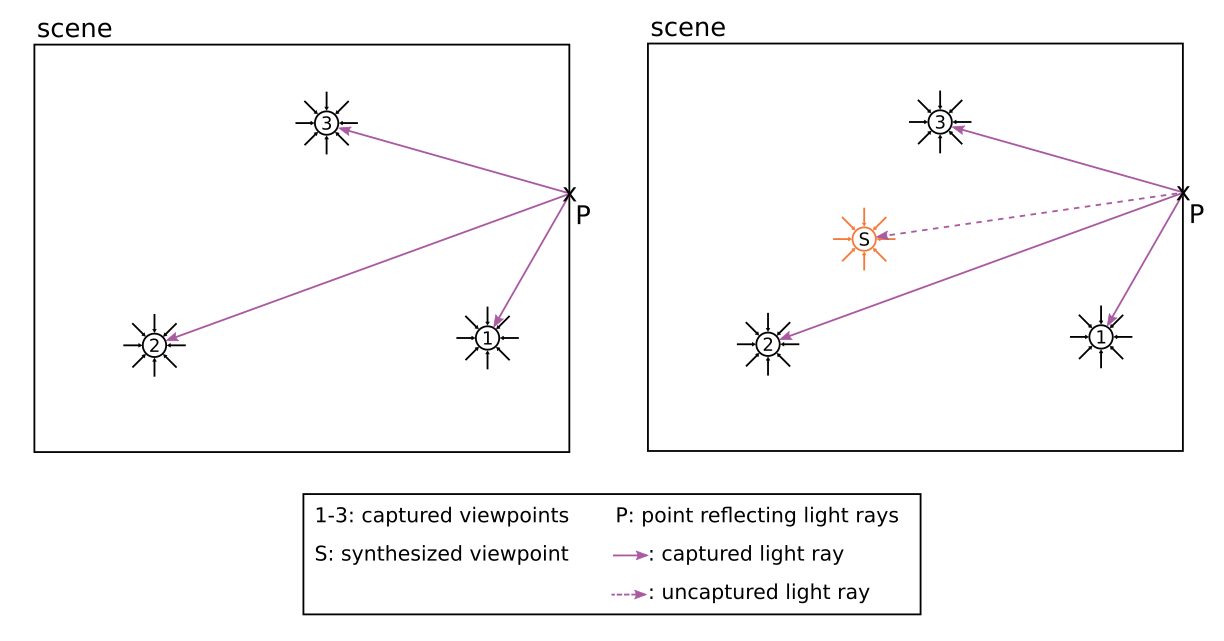
\includegraphics[width=1\textwidth]{03/incoming_lightrays.png}
%\caption[Light rays reflected from a point in the scene]{The reflected light rays from each point in the scene are captured by each 360\degree viewpoint}
%\label{fig:reflected_rays}
%\end{figure}

%\begin{itemize}
%    \item all viewpoints more or less capture complete surroundings from different perspectives \ar each point from an input viewoint will be somewhere on the synthesized viewpoint
%    \item find corresponding points with the output viewpoint for each input viewpoint (\emph{``where would point P (seen in viewpoint A) be in the synthesized viewpoint S''})
%    \item to determine which viewpoints to use for which output image areas, use weighting function $W(viewpoint)$ that is dependent on specific properties of the input viewpoint (e.g. euclidean distance of locations)
%    \item in order to do all this, need scene model which is a sphere since we have no geometry information
%\end{itemize}

%The main difference between 1DoF and 2/3DoF synthesis is that in 1DoF interpolation, the choice of viewpoints is trivial, as there are only two by definition. In 2/3DoF synthesis, the idea is to have an unlimited number of viewpoints as input (for 2DoF synthesis, these viewpoints must all be on a plane). Since all the images are 360\degree images, each one theoretically captures the complete surroundings. This means that every existing point should be present somewhere in each image (ignoring occlusions at the moment).
%The basic idea of the 2/3DoF algorithm is to find the image areas from the set of existing viewpoints that are the ``most fitting'' for the synthesized viewpoint and transform these areas to approximate where they would be in the synthesized image. This means that a metric is necessary that measures how ``fitting'' a specific pixel of a viewpoint image is. Also, a reprojection needs to be found that transforms the ``fitting'' image areas to the appropriate image coordinates for the synthesized viewpoint.
%\missingfigure{point correspondences and reprojection intro}


\subsubsection{Deviation angle constraint}
- different sections of different viewpoints may be more appropriate in terms of accuracy
- use deviation angle as constraint (other possibilities are also possible, such as a combination of deviation angle and distance)
- calculate deviation angle and blend the best 2 based on a blending function (inverse sigmoid)

%In order to find the ``most fitting'' image area from all of the viewpoint images, there first needs to be a metric that measures how ``fitting'' an image area is. 

%One example is the euclidean distance of the viewpoint locations in space. This would mean that for each pixel, the corresponding pixel of the \emph{nearest viewpoint} would be used. This is the simplest approach, and would simply return the nearest neighbor. 

\subsection{2DoF Synthesis using Flow-based Blending}
- using only basic 2DoF synthesis works fairly well as long as the actual geometry of the scene corresponds more or less to the model geometry (sphere)
- ghosting/aliasing problems as soon as objects are closer or farther than the sphere radius
- use flow-based blending from Megastereo to improve this

%The simplest type of synthesis in the scope of this thesis is the creation of a new viewpoint that lies exactly on a line between two existing viewpoints. Assuming that the existing viewpoints are facing the same direction, the line describes a transformation with one degree of freedom, i.e. movement along the line. A solution to a similar problem has already been published by Richardt et al. in ``Megastereo'' \cite{megastereo} which introduces an approach using optical flow in order to reduce ghosting artefacts in planar images. The following section shows how the problem of 1D interpolation for 360\degree images can be reduced to the problem solved in Megastereo.

\subsubsection{Flow-based Blending in Megastereo}
%Megastereo aims to generate high-resolution stereo panoramas by combining images captured on a circle. Their approach is to combine corresponding strips of the captured images and to create a view for each eye (see section \ref{megastereo}). In order to mitigate artefacts such as ghosting, they use ``flow-based blending'' to combine two images A and B. This consists of using the optical flow vectors $F_{A\rightarrow B}$ and their inverse $F_{B\rightarrow A}$. To get the interpolated image at position $\alpha$ between image A and B, first, image A is shifted by $\alpha \cdot F_{A\to B}$ and image B is shifted by $(1 - \alpha) \cdot F_{A\to B}$, yielding $I_A$ and $I_B$, respectively. Then, $I_A$ is multiplied by $(1-\alpha)$ and $I_B$ by $\alpha$ and these pixel values are added together to give the resulting interpolation. This is described by the following function, in which each pixel at position x is defined by: 
%\begin{align}
%S(x) = (1-\alpha ) \cdot I_A( x + \alpha \cdot F_{A\to B}(x) \\
%     + \alpha \cdot I_B( x + (1-\alpha) \cdot F_{B\to A}(x))
%\end{align}

\subsubsection{Reducing 360\degree Interpolation to Planar Interpolation}

A 360\degree image can be projected in several ways, as described in Section \ref{projections}. The output of these projections is a planar image, meaning that flow-based blending could be applied directly. However, this would not lead to optimal results for several reasons: Most projections distort the image in some areas, which would result in distorted optical flow values. Furthermore, in order to make planar viewing possible, the 360\degree image must be ``unfolded'' along some seam. When calculating optical flow, points that move across the seam will not be tracked, even though they do not move out of the image space, as would happen in a regular image.
\missingfigure{points moving across edge in regular vs 360\degree image}

Of the existing projections, only two really come into consideration for this problem: the equirectangular representation and the cubemap representation. Spherical representations are impractical, as aligning seams is not feasible. The equirectangular representation has fewer seams to handle, but also distorts the image greatly around the poles. The cubemap representation hardly distorts the image at all, but contains a number of seams. In this case, the distortion is more difficult to deal with, since the effects on the optical flow algorithm are unclear. Handling seams is more straightforward, which is why the cubemap representation was chosen for 1D interpolation.

In order to handle points moving across seams, the optical flow algorithm must be able to read data \emph{across the seams}. For example, when calculating optical flow on the ``front'' face, data from the ``top'', ``left'', ``right'' and ``bottom'' faces is required. Intuitively, one might just assemble these faces in a plus shape, with the ``front'' face at the center. However, this is a fallacy, since the cubemap projection uses a different virtual camera for each face, which means that linearity is not preserved for points moving across seams.

\missingfigure{cubemap with point moving across seam}

To solve this problem, the ``extended cube map'' is introduced, which was also used by Huang et. al. \cite{6dof}. Instead of projecting a field of view of 90\degree for each camera, which covers 360\degree of the image, the extended cube map uses a larger field of view for each camera. As a result, the areas of the image that are split by a seam are represented twice: Once on each face that is adjacent to the seam. This way, when calculating optical flow on each face separately, points that move across where the seam would be in a regular cube map remain on the face with the corresponding projection. 

Naturally, this method is limited by the field of view used by the virtual cameras. If the maximum displacement is larger than the face extension, the extended cube map will not be sufficient, which will result in black edges on the faces. Also, the larger the field of view, the more the image will be distorted towards the edges of a face, which may lead to distorted optical flow results. This means that displacement between two images is limited. However, the displacement that is trackable by optical flow algorithms is also limited. The effect of these limitations will be explored in section \ref{evaluation1D}.

Using the extended cube map, it is possible to process each face separately, meaning that the 360\degree 1DoF interpolation has been reduced to planar images. At the end of the interpolation step, the extended cube map must be clipped back to the original cube map size.
\missingfigure{1D interpolation process diagram}

%further points to include
%- inverting flow is non-trivial

\section{Implementation}

\subsubsection{Preprocessing and CaptureSet}
\begin{itemize}
  \item rotate all images so that they all have the same orientation
  \item center point cloud
  \item find appropriate sphere radius
  \item make access to location and image data of a viewpoint contained in a set easy and intuitive
\end{itemize}

\subsubsection{Interpolation}
\begin{itemize}
  \item ray and scene intersection
  \item viewpoint reprojection
  \item deviation angle calculation
  \item weighting function
\end{itemize}

\subsection{Debugging and Verification}
\begin{itemize}
  \item in order to verify correct results and check for bugs, use of the ``checkersphere'' in which the scene model exactly matches the scene \ar reprojection will yield exact results (excluding resolution)
  \item explain why it will yield correct results and why the resolution is not perfect
\end{itemize}

\subsection{Implementation challenges}
``one on each side''
\begin{itemize}
  \item define ``on either side'' for angles: split the circle in two 180\degree halves; one is positive, the other is negative
  \item selection of a viewpoint ``on either side'' \ar what if the viewpoint on one side has a very large deviation angle or does not exist?
  \item can it not exist if we are looking at the convex hull? Yes, if the point is exctly on the border
  \item possible solution: if none is found, use only one side
  \item what to do with zero degree difference? \ar only use zero, not the other (should be solved by the function that defines the 1D interpolation position)
\end{itemize}
using only 2D data
\begin{itemize}
  \item ``left and right'' only possible in 2D (can use signed angles)
  \item in 3D, finding viewpoint on ``either side'' becomes a lot more complex
  \item reducing viewpoints to 2D is simple, but scene model is still in 3D. simplifying scene model to 2D as well
\end{itemize}

errors that are unrelated to the algorithm:
\begin{itemize}
  \item slight displacement due to ExtendedCubeMap
  \item black edges due to latlong-cube conversion
  \item these need to be taken into account (normalized out)
  \item only an issue for flow-based because flow-based uses conversion, whereas regular does not
\end{itemize}

\subsection{Performance}
